% Options for packages loaded elsewhere
\PassOptionsToPackage{unicode}{hyperref}
\PassOptionsToPackage{hyphens}{url}
%
\documentclass[
]{book}
\title{Introduction to Statistics}
\author{Aaron McMurray}
\date{2022-06-08}

\usepackage{amsmath,amssymb}
\usepackage{lmodern}
\usepackage{iftex}
\ifPDFTeX
  \usepackage[T1]{fontenc}
  \usepackage[utf8]{inputenc}
  \usepackage{textcomp} % provide euro and other symbols
\else % if luatex or xetex
  \usepackage{unicode-math}
  \defaultfontfeatures{Scale=MatchLowercase}
  \defaultfontfeatures[\rmfamily]{Ligatures=TeX,Scale=1}
\fi
% Use upquote if available, for straight quotes in verbatim environments
\IfFileExists{upquote.sty}{\usepackage{upquote}}{}
\IfFileExists{microtype.sty}{% use microtype if available
  \usepackage[]{microtype}
  \UseMicrotypeSet[protrusion]{basicmath} % disable protrusion for tt fonts
}{}
\makeatletter
\@ifundefined{KOMAClassName}{% if non-KOMA class
  \IfFileExists{parskip.sty}{%
    \usepackage{parskip}
  }{% else
    \setlength{\parindent}{0pt}
    \setlength{\parskip}{6pt plus 2pt minus 1pt}}
}{% if KOMA class
  \KOMAoptions{parskip=half}}
\makeatother
\usepackage{xcolor}
\IfFileExists{xurl.sty}{\usepackage{xurl}}{} % add URL line breaks if available
\IfFileExists{bookmark.sty}{\usepackage{bookmark}}{\usepackage{hyperref}}
\hypersetup{
  pdftitle={Introduction to Statistics},
  pdfauthor={Aaron McMurray},
  hidelinks,
  pdfcreator={LaTeX via pandoc}}
\urlstyle{same} % disable monospaced font for URLs
\usepackage{longtable,booktabs,array}
\usepackage{calc} % for calculating minipage widths
% Correct order of tables after \paragraph or \subparagraph
\usepackage{etoolbox}
\makeatletter
\patchcmd\longtable{\par}{\if@noskipsec\mbox{}\fi\par}{}{}
\makeatother
% Allow footnotes in longtable head/foot
\IfFileExists{footnotehyper.sty}{\usepackage{footnotehyper}}{\usepackage{footnote}}
\makesavenoteenv{longtable}
\usepackage{graphicx}
\makeatletter
\def\maxwidth{\ifdim\Gin@nat@width>\linewidth\linewidth\else\Gin@nat@width\fi}
\def\maxheight{\ifdim\Gin@nat@height>\textheight\textheight\else\Gin@nat@height\fi}
\makeatother
% Scale images if necessary, so that they will not overflow the page
% margins by default, and it is still possible to overwrite the defaults
% using explicit options in \includegraphics[width, height, ...]{}
\setkeys{Gin}{width=\maxwidth,height=\maxheight,keepaspectratio}
% Set default figure placement to htbp
\makeatletter
\def\fps@figure{htbp}
\makeatother
\setlength{\emergencystretch}{3em} % prevent overfull lines
\providecommand{\tightlist}{%
  \setlength{\itemsep}{0pt}\setlength{\parskip}{0pt}}
\setcounter{secnumdepth}{5}
\usepackage{booktabs}
\ifLuaTeX
  \usepackage{selnolig}  % disable illegal ligatures
\fi
\usepackage[]{natbib}
\bibliographystyle{apalike}

\begin{document}
\maketitle

{
\setcounter{tocdepth}{1}
\tableofcontents
}
\hypertarget{Introduction-to-Statistics}{%
\chapter*{Introduction to Statistics}\label{Introduction-to-Statistics}}
\addcontentsline{toc}{chapter}{Introduction to Statistics}

\textbf{Overview}

This resource is intended to provide an introduction to the basics of statistics.

\textbf{Contents}

\begin{itemize}
\tightlist
\item
  Introduction
\item
  Data Types and Levels of Measurement
\item
  Describing Data
\item
  Comparing Data
\item
  Data Visualisation
\item
  Correlation
\item
  Sampling
\item
  Confidence Intervals
\item
  Hypothesis Testing
\item
  Statistical Significance
\item
  Odds against Chance Fallacy
\item
  Statistical Significance Verses Importance
\end{itemize}

\hypertarget{intro}{%
\chapter{Introduction}\label{intro}}

\hypertarget{what-is-statistics}{%
\section{What is Statistics?}\label{what-is-statistics}}

Statistics is all about the collection, organization, analysis, interpretation and presentation of data. Statistics is used everywhere from opinion polling in politics to predicting the prices of assets. There are two main branches of statistics: descriptive statistics and inferential statistics.

\hypertarget{descriptive-statistics}{%
\section{Descriptive Statistics}\label{descriptive-statistics}}

Descriptive statistics describes or summarises data that have been collected. Measures of central tendency and measures of dispersion are the most important tools.

\hypertarget{inferential-statistics}{%
\section{Inferential Statistics}\label{inferential-statistics}}

Inferential statistical is used to make prediction about a population using information gathered about a sample. Inferential statistics involves hypothesis testing and regression analysis.

\hypertarget{data-types-and-levels-of-measurement}{%
\chapter{Data Types and Levels of Measurement}\label{data-types-and-levels-of-measurement}}

Data can be broadly categorised as \textbf{qualitative} (data relating to qualities or characteristics) or quantitative (numerical data relating to sizes or quantities of things).

We can further categorise \textbf{quantitative} data as being continuous or discrete.

\textbf{Discrete} data involves whole numbers that can't be divided because of what they represent (number of people in a class, number of cars owned). The number of people in a class cannot be 10.5 or 3.14. It must be a whole number because people are not divisible.

\textbf{Continuous} data can be divided and measured to some number of decimal places (height, weight, speed in miles per hour). A person's height can be any number (provided it lies within the range of possible human heights) and can be reported to any number of decimal places (150cm or 150.1cm or 150.12cm) depending on how accurate the measurement tool is.

\begin{figure}
\centering
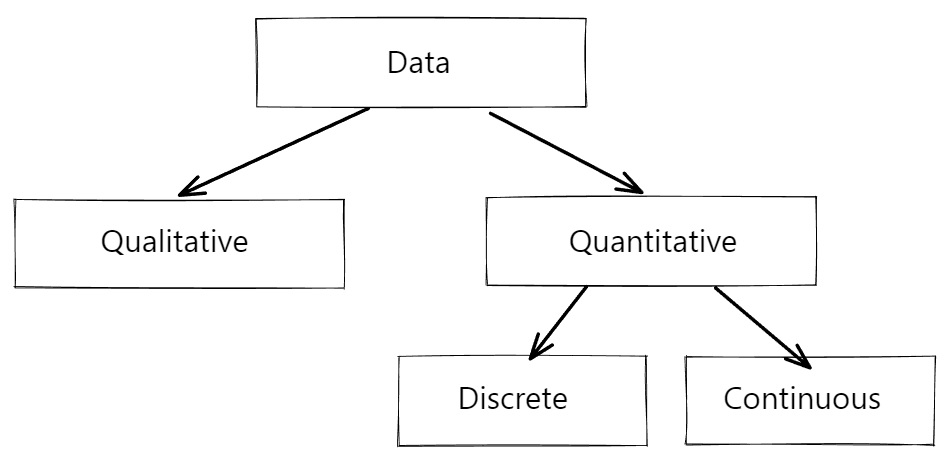
\includegraphics{data.jpg}
\caption{alt text}
\end{figure}

\hypertarget{applications}{%
\chapter{Applications}\label{applications}}

Some \emph{significant} applications are demonstrated in this chapter.

\hypertarget{example-one}{%
\section{Example one}\label{example-one}}

\hypertarget{example-two}{%
\section{Example two}\label{example-two}}

\hypertarget{methods}{%
\chapter{Methods}\label{methods}}

We describe our methods in this chapter.

\hypertarget{final-words}{%
\chapter{Final Words}\label{final-words}}

We have finished a nice book.

  \bibliography{book.bib,packages.bib}

\end{document}
